% Options for packages loaded elsewhere
\PassOptionsToPackage{unicode}{hyperref}
\PassOptionsToPackage{hyphens}{url}
%
\documentclass[
]{article}
\usepackage{amsmath,amssymb}
\usepackage{iftex}
\ifPDFTeX
  \usepackage[T1]{fontenc}
  \usepackage[utf8]{inputenc}
  \usepackage{textcomp} % provide euro and other symbols
\else % if luatex or xetex
  \usepackage{unicode-math} % this also loads fontspec
  \defaultfontfeatures{Scale=MatchLowercase}
  \defaultfontfeatures[\rmfamily]{Ligatures=TeX,Scale=1}
\fi
\usepackage{lmodern}
\ifPDFTeX\else
  % xetex/luatex font selection
\fi
% Use upquote if available, for straight quotes in verbatim environments
\IfFileExists{upquote.sty}{\usepackage{upquote}}{}
\IfFileExists{microtype.sty}{% use microtype if available
  \usepackage[]{microtype}
  \UseMicrotypeSet[protrusion]{basicmath} % disable protrusion for tt fonts
}{}
\makeatletter
\@ifundefined{KOMAClassName}{% if non-KOMA class
  \IfFileExists{parskip.sty}{%
    \usepackage{parskip}
  }{% else
    \setlength{\parindent}{0pt}
    \setlength{\parskip}{6pt plus 2pt minus 1pt}}
}{% if KOMA class
  \KOMAoptions{parskip=half}}
\makeatother
\usepackage{xcolor}
\usepackage[margin=1in]{geometry}
\usepackage{graphicx}
\makeatletter
\def\maxwidth{\ifdim\Gin@nat@width>\linewidth\linewidth\else\Gin@nat@width\fi}
\def\maxheight{\ifdim\Gin@nat@height>\textheight\textheight\else\Gin@nat@height\fi}
\makeatother
% Scale images if necessary, so that they will not overflow the page
% margins by default, and it is still possible to overwrite the defaults
% using explicit options in \includegraphics[width, height, ...]{}
\setkeys{Gin}{width=\maxwidth,height=\maxheight,keepaspectratio}
% Set default figure placement to htbp
\makeatletter
\def\fps@figure{htbp}
\makeatother
\setlength{\emergencystretch}{3em} % prevent overfull lines
\providecommand{\tightlist}{%
  \setlength{\itemsep}{0pt}\setlength{\parskip}{0pt}}
\setcounter{secnumdepth}{-\maxdimen} % remove section numbering
\usepackage{booktabs}
\usepackage{longtable}
\usepackage{array}
\usepackage{multirow}
\usepackage{wrapfig}
\usepackage{float}
\usepackage{colortbl}
\usepackage{pdflscape}
\usepackage{tabu}
\usepackage{threeparttable}
\usepackage{threeparttablex}
\usepackage[normalem]{ulem}
\usepackage{makecell}
\usepackage{xcolor}
\ifLuaTeX
  \usepackage{selnolig}  % disable illegal ligatures
\fi
\IfFileExists{bookmark.sty}{\usepackage{bookmark}}{\usepackage{hyperref}}
\IfFileExists{xurl.sty}{\usepackage{xurl}}{} % add URL line breaks if available
\urlstyle{same}
\hypersetup{
  pdftitle={Manuscript progress report},
  pdfauthor={Ying Jin},
  hidelinks,
  pdfcreator={LaTeX via pandoc}}

\title{Manuscript progress report}
\author{Ying Jin}
\date{2023-12-05}

\begin{document}
\maketitle

{
\setcounter{tocdepth}{3}
\tableofcontents
}
\hypertarget{method}{%
\section{Method}\label{method}}

\hypertarget{assumptions}{%
\subsection{Assumptions}\label{assumptions}}

\begin{itemize}
\tightlist
\item
  For each subject i in the population, a generalized outcome \(Y_i(t)\)
  is generated along a variable t (for example, time), where
  \(t \in (0, T)\).
\item
  The outcome, at any specific t, follows an exponential family
  distribution characterized by a (latent) continuous function
  \(\eta_i(t)\):
\end{itemize}

\[g[E(Y_i(t))] = \eta_i(t) = \beta_0(t)+b_i(t)\]

\[p(Y_i(t)) = h(Y_i(t))exp\{\eta_i(t)T[Y_i(t)]-A(\eta_i(t))\}\]

\begin{itemize}
\tightlist
\item
  The continuous latent function consists of a population-level fixed
  process and an individual-level random process
\end{itemize}

\[\eta_i(t) = \beta_0(t)+b_i(t)\]

\hypertarget{observed-data}{%
\subsection{Observed data}\label{observed-data}}

In practice we would observe the discrete realization of
\(\{Y_i(t), t\}\) along a dense grid. For simplicity, we assume the
observation grid is regular (same across sample). When we have J
observations points in \((0, T]\), then for the jth observation point,
we denote the corresponding value of t as \(t_j\), and the corresponding
outcome at this point \(Y_i(t_j)\).

\hypertarget{fgfpca-algorithm}{%
\subsection{fGFPCA Algorithm}\label{fgfpca-algorithm}}

\hypertarget{bin-data}{%
\subsubsection{Bin data:}\label{bin-data}}

Choose a proper bin width \(w\) considering model complexity and
identifiability. For now let's say the bins are equal-length and
non-overlapping.

\begin{itemize}
\tightlist
\item
  Bin index \(s = 1...S\)
\item
  Index of bin midpoints \(m_s\)
\item
  Value of t corresponding to bin midpoints \(t_{m_s}\)
\item
  Bin endpoints: \((t_{m_s}-\frac{w}{2}, t_{m_s}+\frac{w}{2}]\)
\end{itemize}

\hypertarget{local-glmms}{%
\subsubsection{Local GLMMs}\label{local-glmms}}

At the every bin, we fit a local intercept-only model:

\[g[E(Y_i(t_j))] =\eta_i(t_{m_s})= \beta_0(t_{m_s})+b_i(t_{m_s})\] where
\(t_j \in (t_{m_s}-\frac{w}{2}, t_{m_s}+\frac{w}{2}]\).

Here we are basically saying that the value of latent function is
constant within the same bin, which clearly is a misspecification of the
true latent process.

From the model above. we will be able to estimate a
\(\hat{\eta_i}(t_{m_s})\) on the binned grid for every individual in the
training sample.

\hypertarget{fpca}{%
\subsubsection{FPCA}\label{fpca}}

Here, we fit a FPCA model on the \(\hat{\eta_i}(t_{m_s})\) obtained from
step 2:

\[\hat{\eta}_i(t_{m_s}) = f_0(t_{m_s})+\sum_{k=1}^K\xi_{ik}\phi_{k}(t_{m_s})+\epsilon_i(t_{m_s})\]

where \(\xi_{ik}\) independently follows normal distribution
\(N(0, \lambda_k)\), and \(\epsilon_i(t_{m_s})\) at each point follows
\(N(0, \sigma_2)\).

From this model, we will be able to obtain the following estimates which
are shared across population:

\begin{itemize}
\tightlist
\item
  Population mean \(\hat{f_0}(t_{m_s})\)
\item
  Basis functions
  \(\hat{\mathbf{\Phi}} = \{\hat{\phi}_1(t_{m_s}), ...,\hat{\phi}_K(t_{m_s}))\}\)
\item
  Estimates of variance of scores \(\hat{\lambda}_1...\hat{\lambda}_K\)
\end{itemize}

\hypertarget{projection-and-debias}{%
\subsubsection{Projection and Debias}\label{projection-and-debias}}

The mean and basis functions are evaluated on the binned grid. To extend
it to the original measurement grid data was collected on, we project
the estimated eigenfunctions \(\hat{\mathbf{\Phi}}\) back use spline
basis. Now we have extend the \(\hat{\phi}_k(t_{m_s})\) to the original
grid \(\hat{\phi}_k(t_j)\)

Because of the misspecification of local GLMMs, the estimated
eigenfunctions and eigenvalues are also biased by a constant
multiplicative effect. Therefore, we use a GLMM to re-evaluate the mean
function, eigenfunctions and eigenvalues.

\hypertarget{out-of-sample-prediction}{%
\subsection{Out-of-sample prediction}\label{out-of-sample-prediction}}

Now, let's assume we have a new subject \(u\) with \(J_u\) observations
(\(J_u < J\)). Then the log-likelihood of this new subject would be:

\[l_u=\sum_{t_j<t_{J_u}}log(h(Y_u(t_j)))+\hat{\eta}_u(t_j)T(Y_u(t_j))-log(A[\hat{\eta}_u(t_j)])\]

where
\(\hat{\eta}_u(t_j) = \hat{f}_0(t_j)+\sum_{k=1}^K \xi_{uk}\hat{\phi}(t_j)\).

With estimates for the population-level parameters from fGFPCA
algorithms above, we can estimate \(\xi_{uk}\) by maximization of
\(l_u\). Direct maximization some times does not have closed form
solution. Numeric maximization methods seem not very stable as well. So
I have decided to used a Bayes approach (Laplace Approximation):

\begin{itemize}
\tightlist
\item
  Prior distribution: \(\xi_{uk} \sim N(0, \hat{\lambda}_k)\)
\item
  Posterior distribution: the likelihood of
  \(l_u =l(Y_u(t_j)|\mathbf{\xi}_u)\)
\end{itemize}

Laplace Approximation would get the posterior mode of \(\xi_{uk}\)
through quadratic approximation.

\hypertarget{larger-scale-simulation}{%
\section{Larger-scale simulation}\label{larger-scale-simulation}}

\hypertarget{simulation-set-up}{%
\subsection{Simulation set up}\label{simulation-set-up}}

Here we simulate binary data from cyclic latent process:

\[\begin{aligned}
Y_i(t) & \sim Bernoulli(\frac{exp(\eta_i(t))}{1+exp(\eta_i(t))}) \\
\eta_i(t) &= f_0(t)+ \xi_{i1}\sqrt{2}sin(2\pi t)+\xi_{i2}\sqrt{2}cos(2\pi t)+\xi_{i3}\sqrt{2}sin(4\pi t)+\xi_{i4}\sqrt{2}cos(4\pi t)
\end{aligned}\]

where:

\begin{itemize}
\tightlist
\item
  \(t\) is 1000 equal-spaced observations points on \([0, 1]\) (J =
  1000).
\item
  \(f_0(t)=0\)
\item
  \(\xi_k \sim N(0, \lambda_k)\), and
  \(\lambda_k = 1, 0.5, 0.25, 0.125\) for k = 1, 2, 3, 4 respectively.
\item
  Sample size \(N = 500\)
\item
  In the binning step, we bin every 10 observations
\item
  500 simulations were implemented
\end{itemize}

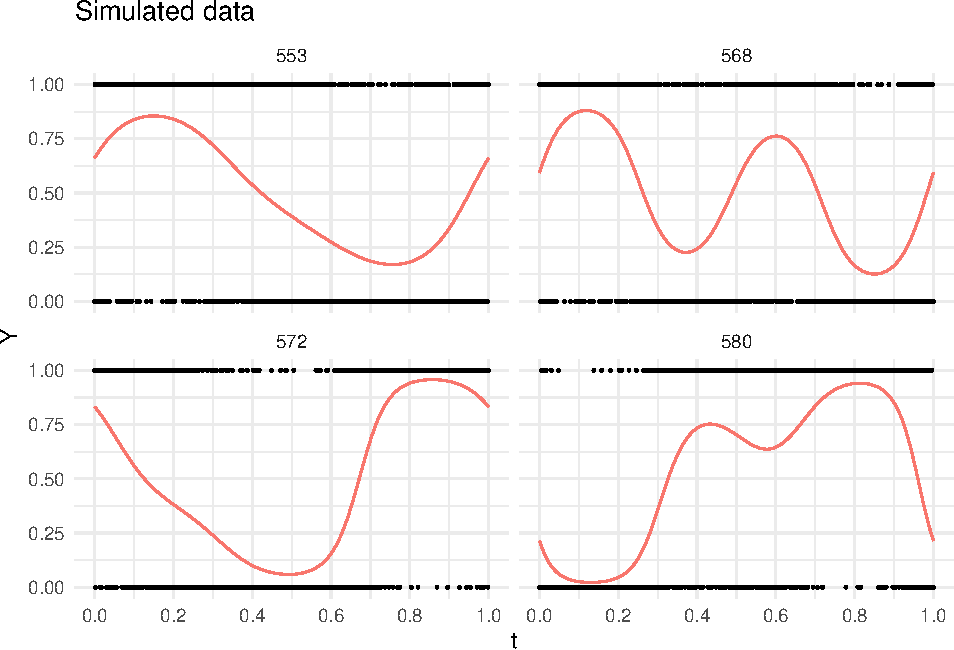
\includegraphics{manuscript_files/figure-latex/fig_sim_data-1.pdf}

\hypertarget{reference-method}{%
\subsection{Reference method}\label{reference-method}}

\begin{itemize}
\tightlist
\item
  GLMMadaptive
\item
  Here we can fit a model with random intercept and slope for time. It
  is doable on 500 datasets, but obviously too simple for the data
  generation scheme. We would expect it to perform terribly.
\end{itemize}

\[g(E(Y_i(t))) = \beta_0+\beta_1t+b_{i0}+b_{i1}t\]

\hypertarget{figure}{%
\subsection{Figure}\label{figure}}

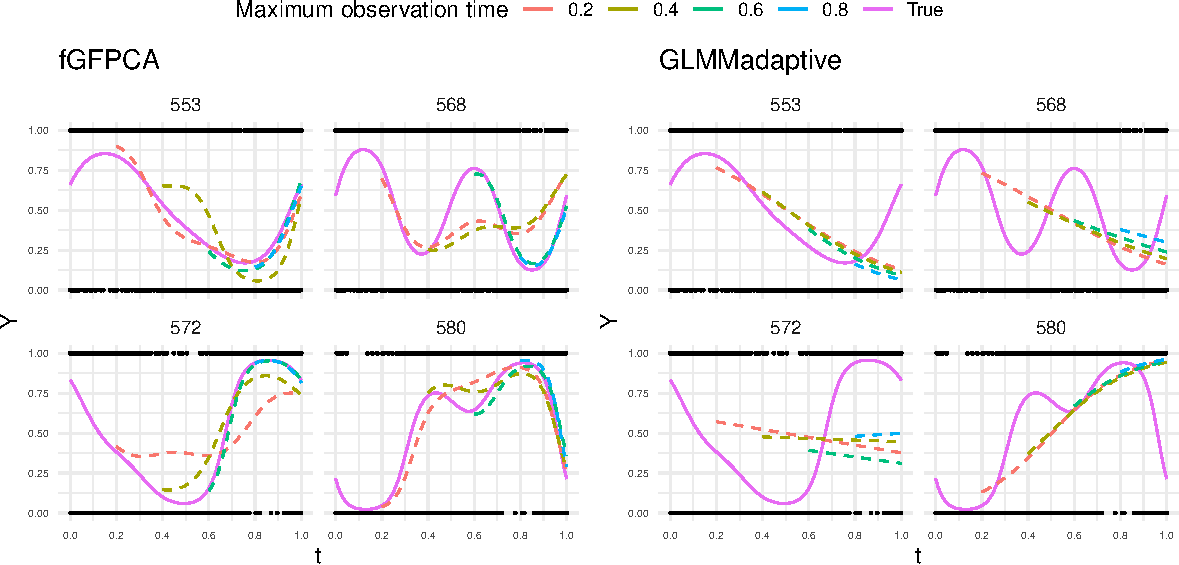
\includegraphics{manuscript_files/figure-latex/fig_sim-1.pdf}

\hypertarget{ise}{%
\subsection{ISE}\label{ise}}

\begin{table}

\caption{\label{tab:unnamed-chunk-4}Integrated squared error}
\centering
\begin{tabular}[t]{lrrrrrrrr}
\toprule
\multicolumn{1}{c}{ } & \multicolumn{8}{c}{Maximum observation time} \\
\cmidrule(l{3pt}r{3pt}){2-9}
\multicolumn{1}{c}{ } & \multicolumn{4}{c}{fGFPCA} & \multicolumn{4}{c}{GLMMadaptive} \\
\cmidrule(l{3pt}r{3pt}){2-5} \cmidrule(l{3pt}r{3pt}){6-9}
Window & 0.2 & 0.4 & 0.6 & 0.8 & 0.2 & 0.4 & 0.6 & 0.8\\
\midrule
(0.2, 0.4] & 146.407 &  &  &  & 387.708 &  &  & \\
(0.4, 0.6] & 183.967 & 74.977 &  &  & 291.579 & 269.799 &  & \\
(0.6, 0.8] & 218.265 & 49.275 & 15.776 &  & 315.778 & 282.736 & 278.242 & \\
(0.8, 1.0] & 108.918 & 77.981 & 17.747 & 12.005 & 563.011 & 477.485 & 597.746 & 600.34\\
\bottomrule
\end{tabular}
\end{table}

\hypertarget{auc}{%
\subsection{AUC}\label{auc}}

\begin{table}

\caption{\label{tab:unnamed-chunk-6}Area under the ROC curve}
\centering
\begin{tabular}[t]{lrrrrrrrr}
\toprule
\multicolumn{1}{c}{ } & \multicolumn{8}{c}{Maximum observation time} \\
\cmidrule(l{3pt}r{3pt}){2-9}
\multicolumn{1}{c}{ } & \multicolumn{4}{c}{fGFPCA} & \multicolumn{4}{c}{GLMMadaptive} \\
\cmidrule(l{3pt}r{3pt}){2-5} \cmidrule(l{3pt}r{3pt}){6-9}
Window & 0.2 & 0.4 & 0.6 & 0.8 & 0.2 & 0.4 & 0.6 & 0.8\\
\midrule
(0.2, 0.4] & 0.748 &  &  &  & 0.591 &  &  & \\
(0.4, 0.6] & 0.664 & 0.734 &  &  & 0.524 & 0.596 &  & \\
(0.6, 0.8] & 0.715 & 0.790 & 0.803 &  & 0.669 & 0.694 & 0.687 & \\
(0.8, 1.0] & 0.740 & 0.755 & 0.781 & 0.784 & 0.514 & 0.556 & 0.526 & 0.564\\
\bottomrule
\end{tabular}
\end{table}

\begin{table}

\caption{\label{tab:time}Computation time (minutes)}
\centering
\begin{tabular}[t]{lrr}
\toprule
Method & Fit & Prediction\\
\midrule
fGFPCA & 0.725 & 1.592\\
GLMMadaptive & 2.287 & 0.017\\
\bottomrule
\end{tabular}
\end{table}

I think we could say that while the total time spend on model fitting +
prediction are similar between two methods, fGFPCA achieved much better
flexibility and much better predictive performance of prediction under
every scenario.

\hypertarget{small-scale-simulation-one-iteration}{%
\section{Small-scale simulation: one
iteration}\label{small-scale-simulation-one-iteration}}

Here we would like to fit fGFPCA and GLMMadaptive on a dataset with
smaller sample size and/or smaller measurement density. For the
GLMMadaptive model, we would set it up with spline basis functions so
that its flexibility is comparable with fGFPCA model, such as:

\[g(E(Y_i(t))) = \sum_{k=1}^4\zeta_{k}B_k(t)+\sum_{l=1}^4\xi_{il}\phi_l(t)\]

I have used 100 subjects for training and testing. When fitting
GLMMadpative, I reduce the number of measurements to 1/10 by taking one
every 10 observations. The prediction is on the original grid.

\hypertarget{figure-1}{%
\subsection{Figure}\label{figure-1}}

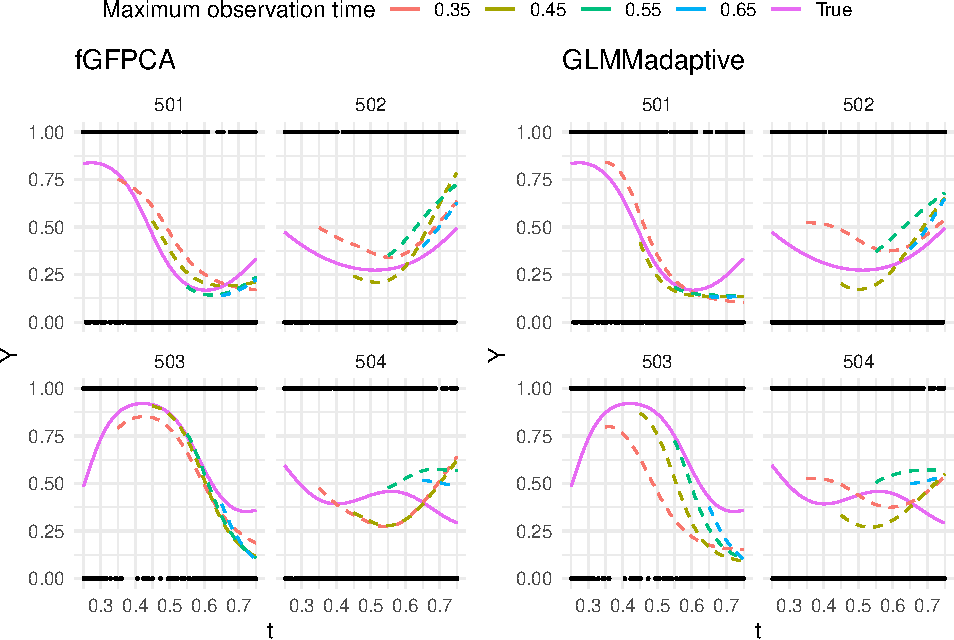
\includegraphics{manuscript_files/figure-latex/unnamed-chunk-7-1.pdf}

\hypertarget{ise-1}{%
\subsection{ISE}\label{ise-1}}

\begin{table}

\caption{\label{tab:unnamed-chunk-8}Integrated squared error}
\centering
\begin{tabular}[t]{l|r|r|r|r|r|r|r|r}
\hline
\multicolumn{1}{c|}{ } & \multicolumn{8}{c}{Observation track} \\
\cline{2-9}
\multicolumn{1}{c|}{ } & \multicolumn{4}{c|}{fGFPCA} & \multicolumn{4}{c}{GLMMadaptive} \\
\cline{2-5} \cline{6-9}
Window & 0.2 & 0.4 & 0.6 & 0.8 & 0.2 & 0.4 & 0.6 & 0.8\\
\hline
(0.2,0.4] & 154.178 &  &  &  & 387.140 &  &  & \\
\hline
(0.4,0.6] & 168.881 & 70.248 &  &  & 248.395 & 415.355 &  & \\
\hline
(0.6,0.8] & 235.562 & 47.770 & 16.813 &  & 330.585 & 321.804 & 265.975 & \\
\hline
(0.8, 1.0] & 97.413 & 77.682 & 19.947 & 12.015 & 186.022 & 525.561 & 349.314 & 116.319\\
\hline
\end{tabular}
\end{table}

\hypertarget{auc-1}{%
\subsection{AUC}\label{auc-1}}

\begin{table}

\caption{\label{tab:unnamed-chunk-9}Integrated squared error}
\centering
\begin{tabular}[t]{l|r|r|r|r|r|r|r|r}
\hline
\multicolumn{1}{c|}{ } & \multicolumn{8}{c}{Observation track} \\
\cline{2-9}
\multicolumn{1}{c|}{ } & \multicolumn{4}{c|}{fGFPCA} & \multicolumn{4}{c}{GLMMadaptive} \\
\cline{2-5} \cline{6-9}
Window & 0.2 & 0.4 & 0.6 & 0.8 & 0.2 & 0.4 & 0.6 & 0.8\\
\hline
(0.2,0.4] & 0.721 &  &  &  & 0.646 &  &  & \\
\hline
(0.4,0.6] & 0.658 & 0.725 &  &  & 0.620 & 0.665 &  & \\
\hline
(0.6,0.8] & 0.710 & 0.793 & 0.805 &  & 0.682 & 0.700 & 0.733 & \\
\hline
(0.8, 1.0] & 0.712 & 0.725 & 0.761 & 0.764 & 0.647 & 0.582 & 0.657 & 0.725\\
\hline
\end{tabular}
\end{table}

There is huge difference in compuation time. GLMMadaptive took 23
minutes, while fGFPCA took less than 3 seconds.

\hypertarget{nhanes-data-application}{%
\section{NHANES data application}\label{nhanes-data-application}}

We take 80\% (7010) subjects for training, 20\% (1753) for out-of-sample
prediction.

In the GLMMadaptive model, I could only fit a model with random
intercept. It took more than 20 minutes for model fitting.

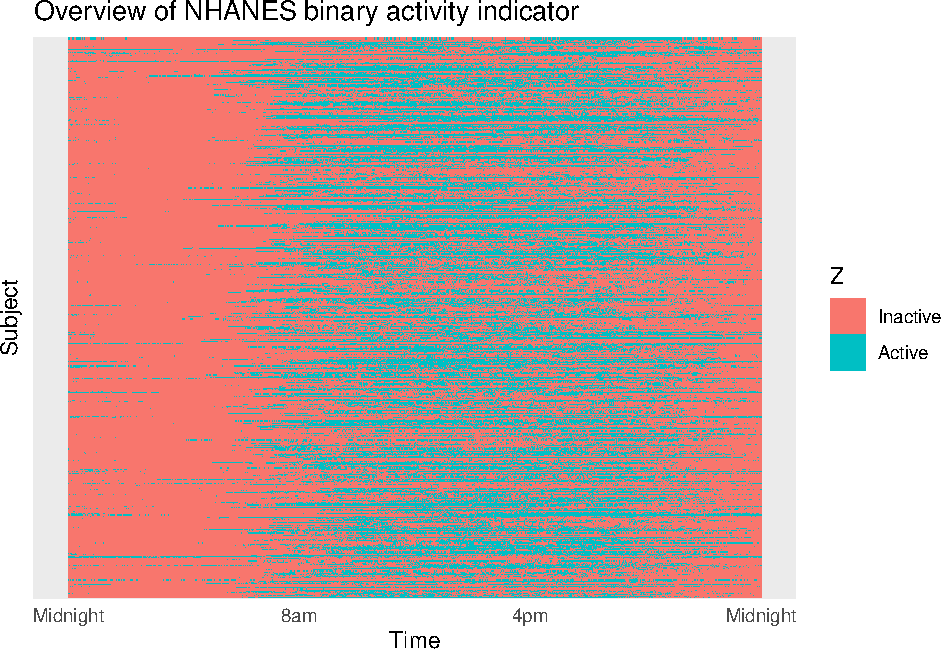
\includegraphics{manuscript_files/figure-latex/nhance_example-1.pdf}

\hypertarget{auc-2}{%
\subsection{AUC}\label{auc-2}}

\begin{table}

\caption{\label{tab:unnamed-chunk-10}Area Under the ROC curve}
\centering
\begin{tabular}[t]{lrrrr}
\toprule
\multicolumn{1}{c}{ } & \multicolumn{4}{c}{Maximum observation time} \\
\cmidrule(l{3pt}r{3pt}){2-5}
\multicolumn{1}{c}{ } & \multicolumn{2}{c}{fGFPCA} & \multicolumn{2}{c}{GLMMadaptive} \\
\cmidrule(l{3pt}r{3pt}){2-3} \cmidrule(l{3pt}r{3pt}){4-5}
Window & 8am & 4pm & 8am & 4pm\\
\midrule
8am-4pm & 0.587 &  & 0.628 & \\
4am-midnight & 0.680 & 0.766 & 0.448 & 0.613\\
\bottomrule
\end{tabular}
\end{table}

\hypertarget{figure-2}{%
\subsection{Figure}\label{figure-2}}

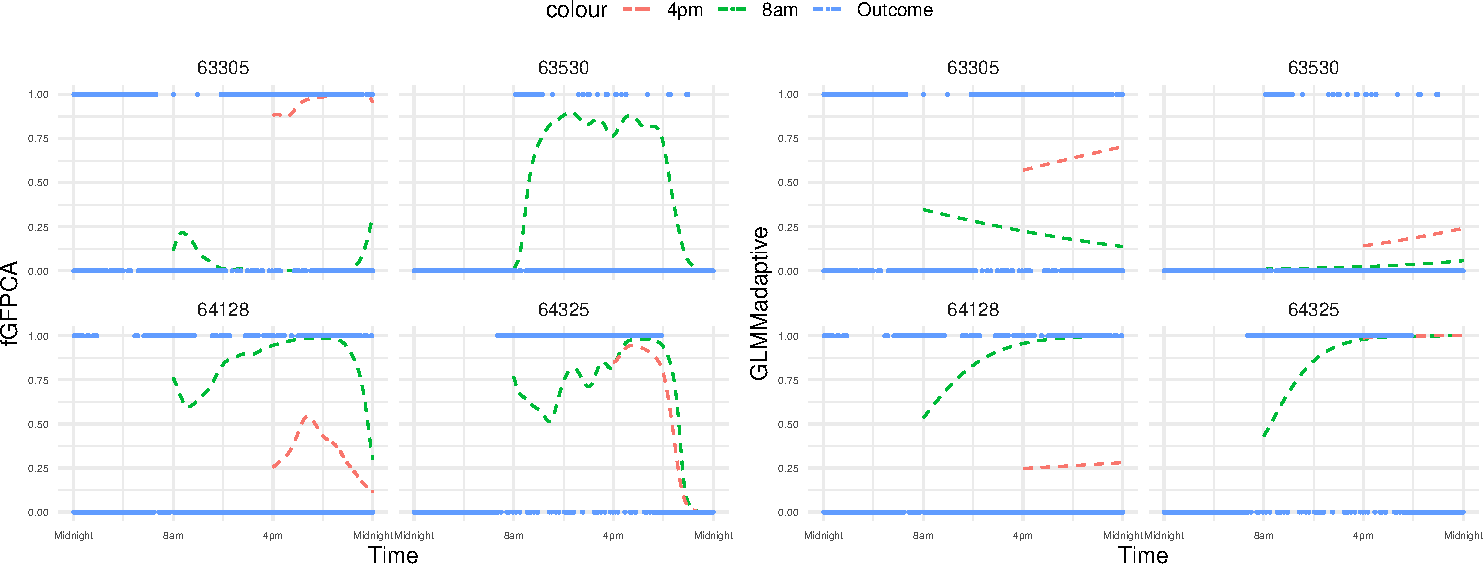
\includegraphics{manuscript_files/figure-latex/pred_nhanes-1.pdf}

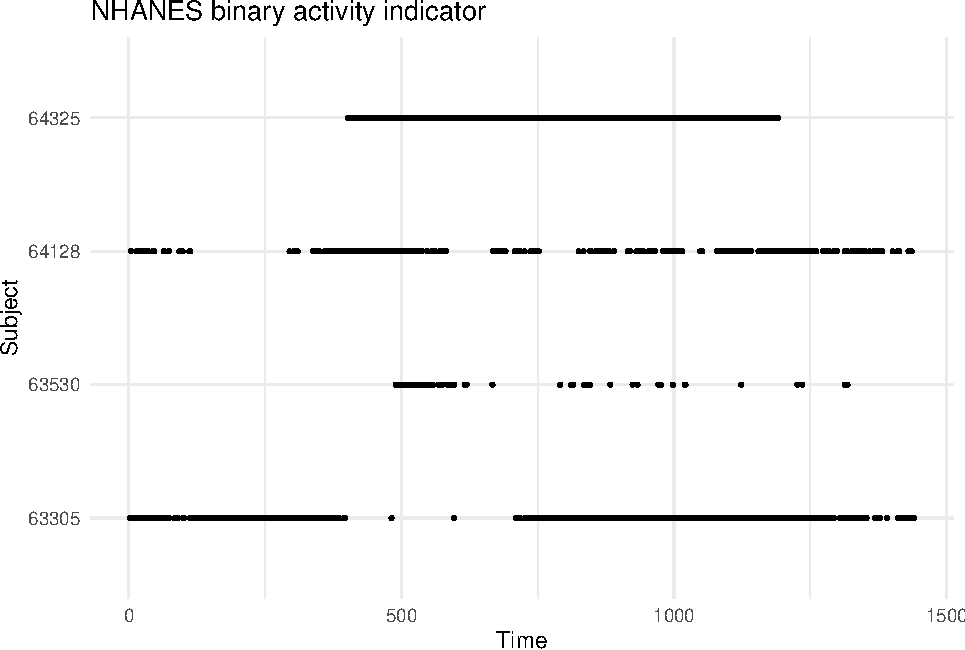
\includegraphics{manuscript_files/figure-latex/small_exp-1.pdf}

\hypertarget{additional-figures}{%
\section{Additional figures}\label{additional-figures}}

\hypertarget{fgfpca-algorithm-demonstration}{%
\subsection{fGFPCA algorithm
demonstration}\label{fgfpca-algorithm-demonstration}}

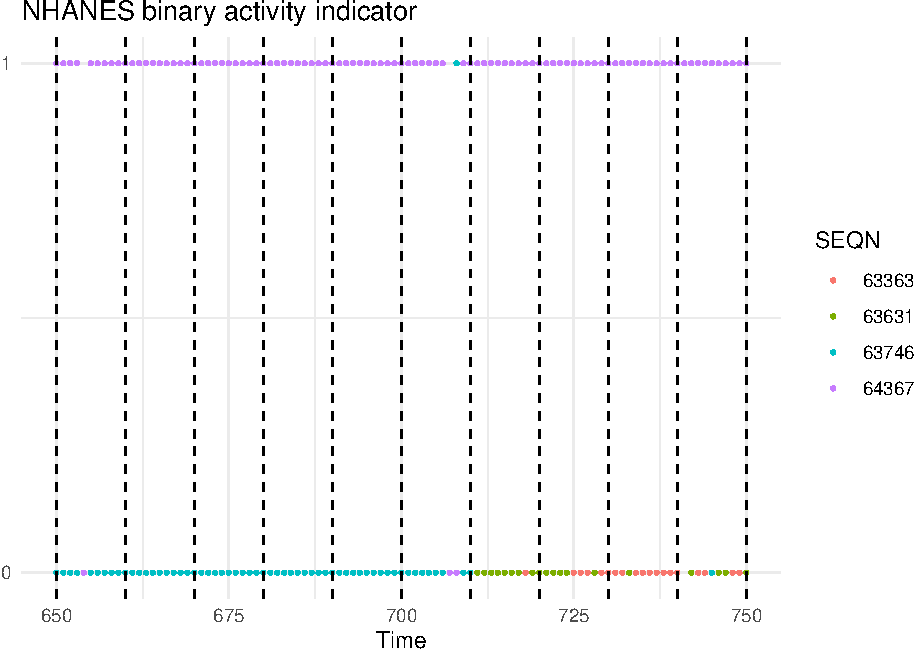
\includegraphics{manuscript_files/figure-latex/binning-1.pdf}

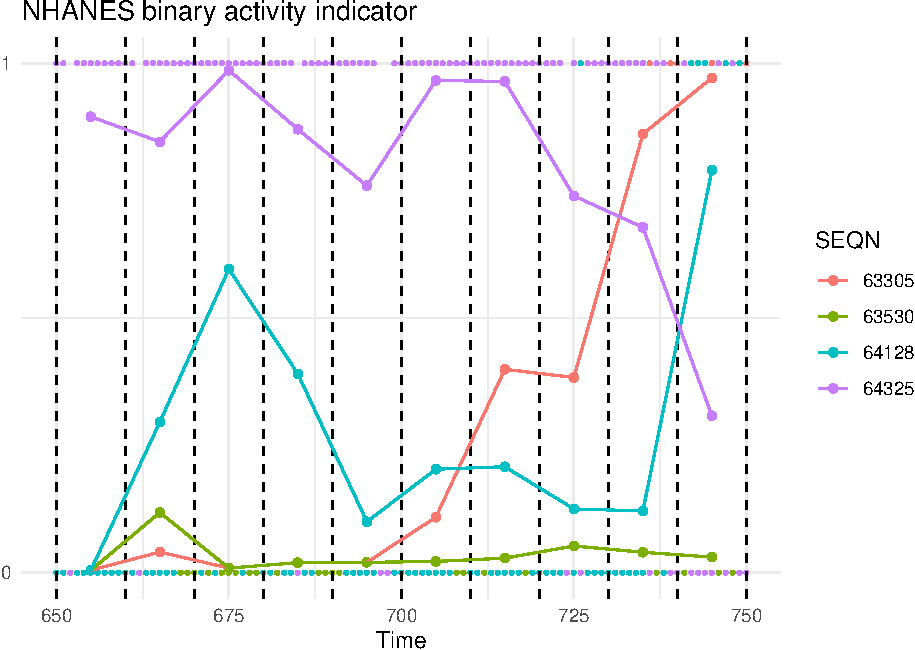
\includegraphics{manuscript_files/figure-latex/unnamed-chunk-11-1.pdf}

\end{document}
